\documentclass[11pt]{beamer}
\newcommand{\R}{\mathbb{R}}
\newcommand{\C}{\mathbb{C}}
\newcommand{\Z}{\mathbb{Z}}
\newcommand{\N}{\mathbb{N}}
\DeclareMathOperator*{\argmin}{arg\,min}
\DeclareMathOperator{\cotan}{cotan}
\DeclareMathOperator{\sinc}{sinc}
\DeclareMathOperator{\Tr}{Tr}
\DeclareMathOperator{\tr}{tr}
\DeclareMathOperator{\Gram}{Gram}
\DeclareMathOperator{\diag}{diag}
\newcommand{\lp}{\left(}
  \newcommand{\rp}{\right)}
\usepackage{blkarray}
\usepackage{multirow}
\usepackage{framed,fancybox}
\usepackage{tikz}
% \usepackage{algorithm2e}
% \usepackage{algorithmic}
\usepackage{float}
\usepackage{framed}
% \usepackage{ulem}
\usetikzlibrary{shapes,arrows}

\newcommand{\lela}{\left \langle}
  \newcommand{\rira}{\right \rangle}
\newcommand{\norm}[1]{\left\lVert#1\right\rVert}
\newcommand{\abs}[1]{\left|#1\right|}

\usepackage{tikz}
\usetikzlibrary{shapes,arrows}
\usepackage[french,english]{babel}
\usepackage[utf8]{inputenc}
\usepackage[T1]{fontenc}
\usepackage{lmodern}
% \usepackage{common}
\usepackage{amsmath,amsfonts,amssymb}
% \usepackage{overpic,boxedminipage}
\usepackage{hyperref}
\usetheme{Warsaw}
\setbeamercolor*{block body alerted}{bg= blue!10}
\setbeamercolor*{block title alerted}{bg= blue!50}
% \usefonttheme{professionalfonts}
\setbeamertemplate{navigation symbols}{}
\setbeamertemplate{headline}{}
\setbeamertemplate{footline}{}
% \setbeamertemplate{blocks}[rounded][shadow=false]
\title[iX_Blue]{Optimisation de trajectoire pour la navigation bathymétrique}
\author{Kieran Delamotte, Carlo de Franchis, David Gontier, Antoine Levitt, Fraçois Madiot, Carlo Marcati}
\date{SEME, Vendredi 16 Janvier 2015}
\institute{Sujet proposé par Jérémy Nicola, iXBlue}
% \institute{CEA, DAM, DIF\\Collaboration avec Marc Torrent}
\newcommand{\loja}{\L{}ojasiewicz\xspace}
\begin{document}

\frame{\titlepage}

\frame{\tableofcontents}
\AtBeginSection[]{
  \begin{frame}{Summary}
    \tableofcontents[currentsection, hideothersubsections]
  \end{frame}
}

\section{Présentation du problème}
\subsection{Contexte}
\frame{
  \frametitle{Positionnement}
  \begin{itemize}
  \item Activité principale de iXBlue : conception de système de
    positionnement pour le pétrolier
  \item Interféromètre à base de fibre optique : donne les
    accélérations selon les six degrés de liberté
    \begin{center}
    \resizebox{.3\textwidth}{!}{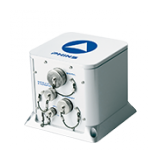
\includegraphics{Images/phins}}
    \resizebox{.5\textwidth}{!}{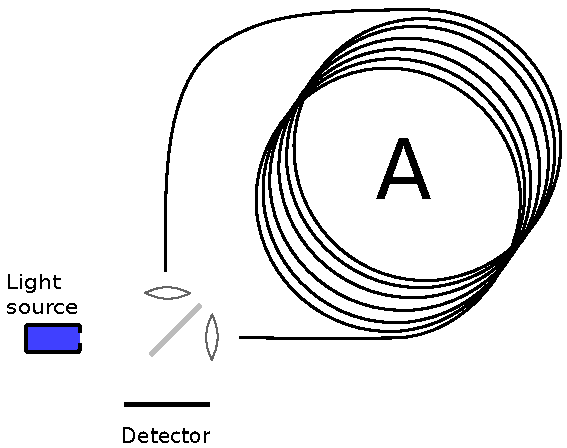
\includegraphics{Images/interferometre}}
  \end{center}
  \end{itemize}

}
\frame{
  \frametitle{Recalage}
  \begin{itemize}
  \item Information locale soumise à dérive. Nécessité d'un recalage
    par des informations globales
  \item Sous-marin : pas possible d'utiliser un GPS
  \item Idée : mesurer le fond marin, et comparer avec des cartes bathymétriques
  \end{itemize}
    \begin{center}
    \resizebox{.6\textwidth}{!}{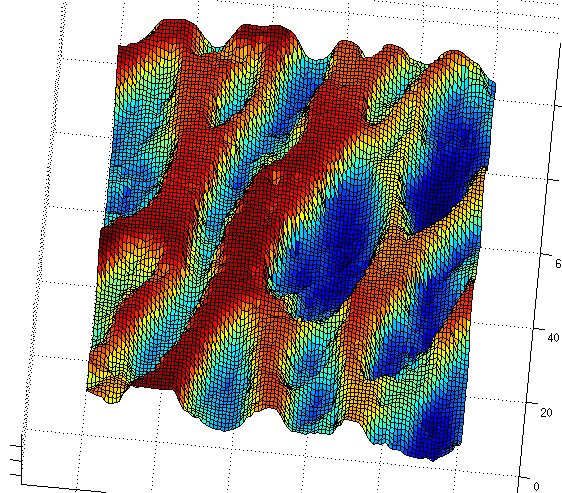
\includegraphics{Images/bathy.png}}
  \end{center}  
}

%%%%%%%%%%%%%%%%%%%%%%%%%
\begin{frame}

\frametitle{Présentation du problème}


\textcolor{red}{Sous-Marin parfait} : 
\begin{itemize}
	\item connait parfaitement la trajectoire de $A$ à $B$.
	\item calcule parfaitement $(v_x(t), v_y(t), h(t))$.
\end{itemize}


\begin{figure}[!h]
\begin{center}
	\begin{tikzpicture}[scale =1]

	%% Boite trajectoire
	\draw (0,0) rectangle (7, 6);
	
	% A et B
	\node at (1, 3.8) {$A$};
	\node at (6, 2.8) {$B$};
	
	% Obstacle
	\foreach \r in {0.1, 0.2, 0.3, 0.5, 0.8}
	{
		\draw (4, 1.5) circle (\r);
	}
		
	\draw[line width=1.5]  (1, 3.5) -- (4, 1.5) -- (6, 2.5);
	\only<1> \shade[ball color=red] (1,3.5) circle (.15);
	\only<2> \shade[ball color=red] (4,1.5) circle (.15);
	\only<3> \shade[ball color=red] (6,2.5) circle (.15);
	

	% temps t
	\only <2> {\draw (10, -0.1) -- (10, 5.8); \node at (10.2, 5.7) {$t$};}
	
	%% Boite vx
	\draw[->] (8, 4) -> (11, 4); 	\draw[->] (8, 4) -> (8, 5.8);	
	\node at (8.3, 5.5) {$v_x$}; \node at (11.2, 4) {$t$};
	
	\only<2-> \draw[red, line width=1.2] (8, 5) -- (10, 5);
	\only<3> \draw[red, line width=1.2] (10,5.4) -- (11, 5.4);
	
	%% Boite vy
	\draw[->] (8, 2) -> (11, 2); 	\draw[->] (8, 2) -> (8, 3.8);
	\node at (8.3, 3.5) {$v_y$}; \node at (11.2, 2) {$t$};
	
	\only<2-> \draw[red, line width=1.2] (8, 2.5) -- (10, 2.5);
	\only<3> \draw[red, line width=1.2] (10,3.4) -- (11, 3.4);
	
	%% Boite h
	\draw[->] (8, 0) -> (11, 0); 	\draw[->] (8, 0) -> (8, 1.8);
	\node at (8.3, 1.5) {$h$}; \node at (11.2, 0) {$t$};
	
	\only<2-> \draw[red, line width=1.2] (8, 0.2) -- (9.4, 0.2);
	\only<2-> \draw[red, line width=1.2]  (9.4,0.2) .. controls (9.7,0.2) and (9.8,1.5) .. (10,1.5);
	\only<3> \draw[red, line width=1.2]  (10,1.5) .. controls (10.2,1.5) and (10.3,0.2) .. (10.6,0.2);
	\only<3> \draw[red, line width=1.2] (10.6, 0.2) -- (11, 0.2);


\end{tikzpicture}
\end{center}
\end{figure}


\end{frame}

\begin{frame}

\frametitle{Présentation du problème}


\textcolor{red}{Sous-Marin réel} : 
\begin{itemize}
	\item connait parfaitement $A$, et la carte de fond.
	\item Il a $(\widetilde{v_x}(t), \widetilde{v_y}(t), \widetilde{h}(t)) = (v_x(t), v_y(t), h(t)) + (e_{v_x}(t), e_{v_y}(t) , e_h(t))$.
	\item \textcolor{red}{But : estimer où est $B$ !}
\end{itemize}

\vspace{-1.5em}

\begin{figure}[!h]
\begin{center}
	\begin{tikzpicture}[scale =1]

	%% Boite trajectoire
	\draw (0,0) rectangle (7, 6);
	
	% A et B
	\node at (1, 3.8) {$A$};
	%\node at (6, 2.8) {$B$};
	
		
	%\draw[line width=1.5]  (1, 3.5) -- (4, 1.5) -- (6, 2.5);
	\only<1> \shade[ball color=red] (1,3.5) circle (.15);
	
	\only <2> {
		\filldraw[fill = blue!20, draw = blue] (2.5, 2.5) circle (0.5);
		\draw[line width=1]  (1, 3.5) -- (2.5, 2.5);
		\node[blue] at (2.5, 3.2) {?};
	}
	\only <3> {
		\filldraw[fill = blue!20, draw = blue] (4, 1.5) circle (0.1);
		\draw[line width=1]  (1, 3.5) -- (4, 1.5);
	}
	\only <4> {
		\filldraw[fill = blue!20, draw = blue] (6, 2.8) circle (0.3);
		\draw[line width=1]  (1, 3.5) -- (4, 1.5) -- (6, 2.8);
		\node[blue] at (6, 3.3) {B ?};
	}
	
	% Obstacle
	\foreach \r in {0.1, 0.2, 0.3, 0.5, 0.8}
	{
		\draw (4, 1.5) circle (\r);
	}

	%% Boite vx
	\draw[->] (8, 4) -> (11, 4); 	\draw[->] (8, 4) -> (8, 5.8);	
	\node at (8.3, 5.5) {$v_x$}; \node at (11.2, 4) {$t$};
	
	\fill[fill=red!20] (8, 4.9) rectangle (10,5.1);
	\draw[red, line width=1] (8, 5) -- (10, 5);
	\fill[fill=red!20](10, 5.3) rectangle (11,5.5);
	\draw[red, line width=1] (10,5.4) -- (11, 5.4);
	
	%% Boite vy
	\draw[->] (8, 2) -> (11, 2); 	\draw[->] (8, 2) -> (8, 3.8);
	\node at (8.3, 3.5) {$v_y$}; \node at (11.2, 2) {$t$};
	
	\fill[fill=red!20] (8, 2.4) rectangle (10,2.6);
	\draw[red, line width=1] (8, 2.5) -- (10, 2.5); 
	\fill[fill=red!20] (10, 3.3) rectangle (11,3.5);
	\draw[red, line width=1] (10,3.4) -- (11, 3.4);
	
	%% Boite h
	\draw[->] (8, 0) -> (11, 0); 	\draw[->] (8, 0) -> (8, 1.8);
	\node at (8.3, 1.5) {$h$}; \node at (11.2, 0) {$t$};
	
	\draw[red!20, line width=6] (8, 0.2) -- (9.4, 0.2);
	\draw[red!20, line width=6]  (9.4,0.2) .. controls (9.7,0.2) and (9.8,1.5) .. (10,1.5);
	\draw[red!20, line width=6]  (10,1.5) .. controls (10.2,1.5) and (10.3,0.2) .. (10.6,0.2);
	\draw[red!20, line width=6] (10.6, 0.2) -- (11, 0.2);
	
	\draw[red, line width=1] (8, 0.2) -- (9.4, 0.2);
	\draw[red, line width=1]  (9.4,0.2) .. controls (9.7,0.2) and (9.8,1.5) .. (10,1.5);
	\draw[red, line width=1]  (10,1.5) .. controls (10.2,1.5) and (10.3,0.2) .. (10.6,0.2);
	\draw[red, line width=1] (10.6, 0.2) -- (11, 0.2);

	%% temps
	\only <2> {\draw (9, -0.1) -- (9, 5.8); \node at (9.2, 5.7) {$t$};}
	\only <3> {\draw (10, -0.1) -- (10, 5.8); \node at (10.2, 5.7) {$t$};}

\end{tikzpicture}
\end{center}
\end{figure}


\end{frame}


% \frame{
%   \frametitle{Choix du chemin}
%   \begin{itemize}
%   \item Comment aller de $A$ en $B$ de façon précise ?
%   \item La ligne droite n'est pas forcément la meilleure
%     stratégie. DESSIN ICI
%   \end{itemize}
% }

\subsection{Notre problème}
\frame{
  \frametitle{Notre problème}
  \begin{center}
    Quel est le chemin de $A$ à $B$ qui minimise l'incertitude en
    $B$ ?
  \end{center}
  \begin{itemize}
  \item Choix du modèle d'incertitudes
  \item Détermination d'une fonction coût
  \item Optimisation de chemin
  \end{itemize}
}

\section{Modélisation et algorithmes de recalage}
\subsection{Approche par intervalles}

\begin{frame}

\frametitle{Enoncé du problème sous forme continue}

On veut trouver la trajectoire initiale (du sous-marin parfait) qui minimise \textcolor{red}{l'incertitude} ($\sim$ "l'aire" finale). \\
~\\
Soit $\gamma_0 \in C^0( [0,T], \R^2)$ la trajectoire du sous-marin parfait, on note $\mathcal{A}_{\gamma_0}$ l'ensemble des \textcolor{red}{trajectoires admissibles}:
\[
	\begin{array}{ll}
		\mathcal{A}_{\gamma_0} :=   \Big\{ &\gamma \in C^0( [0,T], \R^2), \\
			& \gamma(0) = A, \\
			& \forall \ 0 \le t \le T, \quad \left\|  \gamma'(t)  - \gamma_0'(t) \right\|_{\infty} \le \epsilon_v, \\
			& \forall \ 0 \le t \le T, \quad \left| H(\gamma(t))  - H(\gamma_0(t)) \right| \le \epsilon_h. \Big\}
			\end{array}
\]
L'incertitude de $\gamma_0$ est
\[
	c(\gamma_0) = \left| \left\{ \gamma(T), \ \gamma \in \mathcal{A}_{\gamma_0} \right\} \right|.
\]
Le (pseudo)-problème est 
\[
	\argmin \left\{ c(\gamma_0), \ \gamma_0 \in C^0( [0,T], \R^2), \ \gamma_0(0) = A, \ \gamma_0(T) = B \right\}.
\]

\end{frame}

%%%%%%%%%%%%%%%%%%%%%%%%%%%%%%%%%%%%%%%%%%%

%%%%%%%%%%%%%%%%%%%%%%%%%%%%%%%%%%%%%%%%%%%

\begin{frame}

\frametitle{Variantes et énoncé sous forme discrète}


\textcolor{red}{Variantes :}
\begin{itemize}
	\item Le temps final $T$ peut-être libre,
	\item On peut vouloir minimiser \textcolor{red}{l'incertitude globale}, au lieu de l'incertitude finale,
	\item On peut vouloir rajouter des contraintes sur $\gamma_0$, par exemple
	\[
		\forall \ 0 \le t \le T, \quad \left\| \gamma'(t) \right\|_\infty \in [v_{\rm min}, v_{\rm max}].
	\]
\end{itemize}

\textcolor{red}{En pratique, toutes les données sont discrètes :}
\begin{itemize}
	\item Le sous-marin réel prend des mesures avec une certaine fréquence (1Hz, ici, 0.1 Hz)
	\item La carte est "pixellisée" (1 pixel = 1 mètre)
\end{itemize}

\begin{center}
\textcolor{red}{On va chercher des stratégies d'optimisation pour des problèmes discrets.}
\end{center}

\end{frame}


%%%%%%%%%%%%%%%%


\begin{frame}

\frametitle{Outline}


\begin{center}
\textcolor{violet}{
	\huge{Calcul de l'incertitude : l'algorithme de recalage.}}
\end{center}

\end{frame}


%%%%%%%%%%%%%%%%%%%%%%%%%%%%%%%%%%%%%%


\begin{frame}

\frametitle{Algorithme de recalage}


\textcolor{red}{Algorithme de recalage (pour le sous-marin réel) :}\\
\indent \textcolor{blue}{Entrée : } $\gamma_0 := \left\{ A, A_1, A_2, \ldots, A_N = B \right\}$\footnote{Ici, $A_k = \gamma_0(kT/N)$} la trajectoire du sous-marin parfait.\\
\indent \textcolor{blue}{Sortie : } L'incertitude $c(\gamma_0)$.\\
~\\

\textcolor{red}{Idée :}
\begin{itemize}
	\item On pose 
	\[
		J_k := \left\{ \gamma \left(\dfrac{kT}{N} \right), \ \gamma \in \mathcal{A}_{\gamma_0} \right\},
	\]
	l'ensemble des positions admissibles au temps $k$.
	\item On a $J_0 = \{ A \}$, et on peut calculer les $J_k$ par récurrences.
	\item On a $c(\gamma_0) = \sharp \left( J_N \right)$ (\textcolor{blue}{incertitude finale}), ou $c(\gamma_0) = \sum_{k=1}^N \sharp \left( J_k \right)$ (\textcolor{blue}{incertitude globale}).
\end{itemize}



\end{frame}



%%%%%%%%%%%%%%%%%%%%%%%%%%%%%%%%%%%%%%


\begin{frame}

\frametitle{Une étape de recalage}

\begin{figure}[!h]
\begin{center}
\begin{tikzpicture}[scale =1]

	%% Box
	\draw (0,0) rectangle (10, 6);
	
	%% J_k
	\draw[blue] (1,3) circle (0.4);
	\draw[blue] (1, 3.5) circle (0.5);
	\fill[blue!20] (1,3) circle (0.4);
	\fill[blue!20] (1, 3.5) circle (0.5);
	\node[blue] at (1, 4.4) {$J_k$};
	
	
	%%%%%%%%%%%%%%
	%% T(J_{k})
	\only<3, 4, 5> {\draw[blue] (5,1) circle (0.7);
	\draw[blue] (5, 1.5) circle (0.8);
	\fill[blue!20] (5,1) circle (0.7);
	\fill[blue!20] (5, 1.5) circle (0.8);}
	
		%%%%%%%%%%%%%%%%%
	% J_{k+1}
	\only<5-> {
		\fill[red!20] (4.45, 0.6) -- (4.75, 0.33) -- (5.25, 0.33) -- (5.72, 1.85) -- (5.35, 2.22) -- (5, 2.3) -- cycle;
	}
	\only<6> {\node[red] at (5, 2.5) {$J_{k+1}$};}
	
	\only<3> {
	\node[blue] at (5, 2.6) {$T(J_{k})$};
	\draw (1,4) -- (5, 2.3);
	\draw (1,2.6) -- (5, 0.3);}
	
	%% A_k, A_{k+1}
	\draw (0.9, 2.9) -- (1.1, 3.1);
	\draw (0.9, 3.1) -- (1.1, 2.9);
	\node at (1, 3.3) {$A_k$};
	
	\only<2> {\node at (3, 1.7) {${v_k}$};}
	\only <2-> {
	\draw (4.9, 0.9) -- (5.1, 1.1);
	\draw (4.9, 1.1) -- (5.1, 0.9);
	\node at (5, 1.3) {$A_{k+1}$};}
	
	\only<2,3> {
	\draw[->] (1,3) -> (5, 1);}
	
	%%%%%%%%%%%%%%%%%
	% frame 4 : ligne de niveaux
	\only<4, 5> {
	\draw[red] (4.3, 0.2) -- (5.3, 3.3); 
	\draw[red] (4.72, 0.2) -- (6.1, 4.5); 
	\draw[red] (5.2, 0.2) -- (6.2, 3.3); 
	}
	\only <4> {
	\node[red] at (6.1, 4.7) {$\{ H^{-1} (h_{k+1}) \}$};
	\node[red] at (7.2, 3.5) {$\{ H^{-1} (h_{k+1} + \epsilon_h) \}$};
	\node[red] at (4.1, 3.5) {$\{ H^{-1} (h_{k+1} - \epsilon_h) \}$};
	}
\end{tikzpicture}
\end{center}
\end{figure}

\only <1> {On part de l'ensemble $J_k$ (avec $A_k \in J_k$).}
\only <2> {On lit une vitesse $\widetilde{v_k} = v_k + e_{v,k}$, avec $| e_{v,k}| < \epsilon_v$.}
\only <3> {On translate l'ensemble par ${v_k}$, et on prend son $\epsilon_v$-voisinage.}
\only <4> {On lit une hauteur $\widetilde{h_{k+1}} = h_{k+1} + e_{h,k+1}$, avec $| e_{h,k+1} | < \epsilon_h$.}
\only <5> {On prend l'intersection.}
\only <6> {On obtient $J_k$ comme l'intersection de 2 ensembles.}

\end{frame}

%%%%%%%%%%%%%%%%%%%%%%%%%%%%%%%%%

\begin{frame}

\frametitle{Algorithme de recalage sur données réelles}

Put pictures here

\end{frame}



%%%%%%%%%%%%%%%%%%%%%%%%%%%%%%%%%%%%%


\begin{frame}

\frametitle{Algorithme de recalage sur données réelles}

Put pictures here

\end{frame}

%%%%%%%%%%%%%%%%%%%%%%%%%%%%%%%%%%%%%
\subsection{Algorithme de recalage par boites}
\section{Optimisation de trajectoire}
\subsection{Gloutonne}
\subsection{Dijkstra}
\section{Pistes continues}
\subsection{Modèle simple}
\begin{frame}
  \frametitle{Modèle simpliste}
Modèle plus simple ?
\begin{align*}
  \min_{\gamma(0) = A, \gamma(1) = B} \int a |\gamma'|^{2} + b |\nabla
  h \cdot \gamma'|^{2}
\end{align*}
\end{frame}
\subsection{Modèle plus compliqué}
\begin{frame}
  \frametitle{Un modèle un peu plus complexe}
Modèle effectif pour les incertitudes en $x$ et $y$ $\sigma_{x}$ et
$\sigma_{y}$ :
\begin{align*}
  \min_{\gamma(0) = 1, \gamma(1) = B} & \hspace{.5cm}\sigma_{x}(1) + \sigma_{y}(1)\\
  \dot \sigma_{x} &= a - b \sigma_{x} (\partial_{x} h(\gamma(t)))^{2}\\
  \dot \sigma_{y} &= a - b \sigma_{y} (\partial_{y} h(\gamma(t)))^{2}.
\end{align*}

Sous la forme générale d'un contrôle optimal.

Problème : modèle non isotrope, problèmes sur les trajectoires
diagonales. Représentation de l'incertitude par une matrice SDP $A$ ?
\begin{align*}
  \dot A = a A - b (A \nabla h \nabla h^{T} + \nabla h \nabla h^{T} A).
\end{align*}
Problème : $A$ ne reste pas forcément SDP ! Quelle équation pour $A$ ?
\end{frame}
\begin{frame}
  \frametitle{Modélisation probabiliste}
  \begin{itemize}
  \item Approche par intervalles néglige la compensation des erreurs
    et est trop pessimiste : si $X_{n+1} = X_{n} + Y$,
    $Y \sim N(0, 1)$, alors $X_{n} \sim N(0, \sqrt n)$, un intervalle
    à $3\sigma$ donne $X_{n} \in [-3n, 3n]$
  \item Inférence bayésienne ? J'ai une information a priori sur la
    position du sous-marin, et je la mets à jour avec les informations
    de bathymétrie
  \end{itemize}
\end{frame}

\section{Conclusion}
\subsection{Résumé}
\subsection{Modélisation des incertitudes}
\begin{frame}
  \frametitle{Incertitudes}
\begin{itemize}
\item Sources d'incertitude : précision de l'accéléromètre, erreurs
  d'intégration (fréquence finie), erreur numérique (stockage en
  virgule flottante)
\item Dérive de l'estimation de position
\item Modélisation délicate
\item Si on fait une erreur initiale sur l'accélération, dérive en
  $t^{2}$
\item Si on fait une erreur initiale sur la vitesse, dérive en
  $t^{2}$
\item Compensation des erreurs ? Marche aléatoire, dérive en $\sqrt t$
  ? $t^{3/2}$ ? $t^{5/2}$ ?
\end{itemize}
\end{frame}

\begin{frame}
  \frametitle{Modélisation probabiliste}
  \begin{itemize}
  \item Soit $(x_{0}, x_{1} \dots, x_{N})$ le chemin suivi par le
    sous-marin, supposé exact.
  \item Soit $X_{n}$ la position estimée du sous-marin. $X_{n+1}$ ?
  \item Sans bathymétrie, on met à jour la position avec le vecteur
    vitesse $v_{n} = x_{n+1} - x_{n}$, entaché d'une erreur aléatoire
    $\varepsilon_{v}$
  \item La bathymétrie nous donne $h(X_{n+1}) = h(x_{n+1}) +
    \varepsilon_{h}$
  \end{itemize}

  \begin{center}
  \boxed{\mbox{$X_{n+1} \sim L(X_{n} + v_{n} + \varepsilon \;\Big|\;
    h(X_{n} + v_{n} + \varepsilon) = h(x_{n+1}) + \tilde \varepsilon)$}}
  \end{center}
\end{frame}
\begin{frame}
  \frametitle{Modélisation probabiliste}
  \begin{center}
  \boxed{\mbox{$X_{n+1} \sim L(X_{n} + v_{n} + \varepsilon \;\Big|\;
    h(X_{n} + v_{n} + \varepsilon) = h(x_{n+1}) + \tilde \varepsilon)$}}
  \end{center}

  En notant formellement $P(X=x)$ pour la densité de $X$ en $x$,
  \begin{align*}
    P(X_{n+1} = x) &= P(X_{n} + v_{n} + \varepsilon = x \;\Big|\;
    h(X_{n} + v_{n} + \varepsilon) = h(x_{n+1}) + \tilde
                     \varepsilon)\\
    &= \frac 1 N P(X_{n} + v_{n} + \varepsilon = x \cap
    h(X_{n} + v_{n} + \varepsilon) = h(x_{n+1}) + \tilde \varepsilon)\\
    &= \frac 1 N P(X_{n} + v_{n} + \varepsilon = x) \; P(h(x) = h(x_{n+1}) + \tilde \varepsilon),
  \end{align*}
  où $N$ est choisi pour normaliser $X_{n+1}$.
  \begin{itemize}
  \item $P(h(x) = h(x_{n+1}) + \tilde \varepsilon)$ peut être calculé
  \end{itemize}
  

  On peut donc calculer la densité de probabilité de $X_{n+1}$ en
  fonction de $X_{n+1}$ par une translation, une convolution et une multiplication
\end{frame}


\begin{frame}
  \frametitle{Feature detection}
  \begin{itemize}
  \item Si une hauteur $H$ est atteinte en un unique point $(x,y)$,
    alors $(x,y)$ permet de se recaler exactement
  \item Idée : détecter les ``points d'intérêt'' 
  \end{itemize}
\end{frame}

\subsection{Bibliographie}
\end{document}
